\documentclass[sigconf]{acmart} % Removed redundant 'natbib'

% Core Packages - Optimized for XeLaTeX
\ifxetex
  % XeLaTeX handles UTF-8 natively, no need for inputenc
\else
  \usepackage[utf8]{inputenc} % Essential for pdfLaTeX with UTF-8
  \usepackage{fontenc}    % Essential for pdfLaTeX font encoding
\fi

% Essential packages not covered by acmart or providing significant enhancements
% \usepackage{amsmath,amsfonts} % Loaded by acmart
% \usepackage{graphicx} % Loaded by acmart
% \usepackage{booktabs} % Loaded by acmart
% \usepackage{tabularx} % Loaded by acmart
\usepackage{multirow} % For multirow cells in tables (TAPS accepted)
\usepackage{listings} % For code listings (Author choice, TAPS accepted)
% \usepackage{xcolor}   % Loaded by acmart
% \usepackage{url} % Handled by hyperref (loaded by acmart)
\usepackage{xurl} % For better URL line breaking (enhancement over hyperref's default)
\usepackage{algorithm} % For algorithm environment (Author choice, TAPS accepted)
\usepackage{algpseudocode} % For pseudocode in algorithm environment (Author choice, TAPS accepted)
% \usepackage{appendix} % acmart has \appendix command, this package might conflict. Removed.
% \usepackage{balance}  % Loaded by acmart
\usepackage{cleveref} % For smart cross-referencing (Load after hyperref, which acmart loads)
\usepackage{ragged2e} % For better text justification (Use locally and cautiously, acmart enforces full justification)
% \usepackage{setspace} % Loaded by acmart conditionally
% \usepackage{textcomp} % Loaded by acmart
\usepackage{orcidlink} % For ORCID integration
\usepackage{enumitem} % Enhanced list formatting (TAPS accepted)

% Font configuration - acmart handles Libertine and newtxmath loading.
% The following \let\Bbbk\relax and \usepackage{amssymb} are removed as newtxmath should be sufficient.
% \let\Bbbk\relax % May not be needed if amssymb is removed
% \usepackage{newtxmath} % Loaded by acmart with 'libertine' option
% \usepackage{amssymb} % Removed: newtxmath typically covers AMS symbols and avoids conflicts

% Enhanced font configuration for Libertine family with proper XeLaTeX support
\ifxetex
  % For XeLaTeX, use fontspec for better font handling
  \usepackage{fontspec}
  \setmainfont{Linux Libertine O}
  \setsansfont{Linux Biolinum O}
  % Use a more compatible monospace font for XeLaTeX (acmart default is often Inconsolata/zi4)
  % DejaVu Sans Mono is a good alternative if preferred.
  \setmonofont{DejaVu Sans Mono} % Keep user's preferred mono font
\else
  % For other engines (pdfLaTeX), acmart loads libertine and T1 fontenc.
  % Explicit \usepackage{fontenc} moved to top of this \else block.
  % Explicit \usepackage{libertine} removed as acmart handles it.
\fi

% Better Unicode character support for XeLaTeX
\ifxetex
  % For XeLaTeX, direct Unicode input is preferred.
  % Removed redefinitions of \textemdash and \textrightarrow.
  % Removed \catcode changes for '—' and '→' as they are error-prone.
  % Users should input Unicode characters directly (e.g., — for em-dash, → for right arrow).
\else
  % For non-XeLaTeX, ensure standard commands are defined.
  \providecommand{\textemdash}{---} % Standard LaTeX em-dash
  \providecommand{\textrightarrow}{<span class="math-inline">\\rightarrow</span>} % Standard LaTeX right arrow
\fi

% Algorithm line numbering and hyperref compatibility
% Using a standard method to make hyperref targets for algorithm lines unique.
\makeatletter
\ifdefined\theHALG@line % Check if \theHALG@line is defined (by algorithmicx via acmart)
  \renewcommand{\theHALG@line}{\thealgorithm.\arabic{ALG@line}}
\else
  % Fallback or warning if algorithmicx/acmart hasn't set this up as expected
  % This case should ideally not be reached with acmart and algpseudocode.
\fi

% Custom algorithm counter and reset command.
% The utility of algcounter and specific algline... counters needs to be clear.
% ALG@line is reset by algorithmic environment itself.
% If these are for a very specific cross-referencing scheme not covered by standard labels,
% they can be kept, otherwise, they might be an overcomplication.
% For now, retaining the structure but noting its complexity.
\newcounter{algcounter} % User's global algorithm counter
\setcounter{algcounter}{0}

% Unique algorithm line counters for each algorithm (utility needs to be confirmed by user)
\newcounter{alglinegs}
\newcounter{alglinepgc}
\newcounter{alglinevalidation}
\newcounter{alglinesafety}
\newcounter{alglineconflict}
\newcounter{alglinebias}

% Enhanced reset that uses algorithm-specific counters
\newcommand{\resetalglineno}{%
  \stepcounter{algcounter}%
  \setcounter{ALG@line}{0}% Reset standard algorithmicx line counter
  % Reset all algorithm-specific counters (if truly needed for custom referencing)
  \setcounter{alglinegs}{0}%
  \setcounter{alglinepgc}{0}%
  \setcounter{alglinevalidation}{0}%
  \setcounter{alglinesafety}{0}%
  \setcounter{alglineconflict}{0}%
  \setcounter{alglinebias}{0}%
  % Reset other algorithm package counters if they exist (from original code, may not be needed)
  \ifcsname c@algocf@line\endcsname\setcounter{algocf@line}{0}\fi%
  \ifcsname c@ALC@line\endcsname\setcounter{ALC@line}{0}\fi%
}
\makeatother
% The complex \hypertarget patch from original [10] is removed in favor of \theHALG@line redefinition.

% Enhanced microtype configuration
% acmart loads microtype. Explicit setup can fine-tune.
\ifxetex
  % Configure microtype for XeLaTeX - protrusion is the main benefit.
  % expansion, tracking, kerning are generally not handled by microtype with XeTeX or handled by fontspec.
  \microtypesetup{activate={true,nocompatibility},final,expansion=false,tracking=false,kerning=false,spacing=false}
\else
  % Configure microtype for pdfLaTeX (user's original settings, generally good for pdfLaTeX)
  \microtypesetup{activate={true,nocompatibility},final,tracking=true,kerning=true,spacing=true,factor=1100,stretch=10,shrink=10}
\fi

% Consolidated Hyperlink Configuration
\hypersetup{
  pdftitle={AlphaEvolve-ACGS: A Co-Evolutionary Framework for LLM-Driven Constitutional Governance in Evolutionary Computation}, % Matches document title
  pdfauthor={Martin Honglin Lyu},
  pdfsubject={A Co-evolutionary Constitutional Governance Framework for Evolutionary AI, Constitutional AI, Evolutionary Computation, Governance Systems, Policy Synthesis}, % Merged subjects
  pdfkeywords={AI Governance, Evolutionary Computation, Constitutional AI, Large Language Models, Policy-as-Code, Open Policy Agent, Responsible AI, Algorithmic Governance, Dynamic Policy, Co-evolving Systems, Formal Verification, Democratic Governance, SMT Solvers, Algorithmic Fairness}, % Merged and expanded keywords
  pdfcreator={LaTeX with acmart class}, % Consistent
  pdfproducer={pdfTeX}, % Or XeTeX if compiled with XeLaTeX
  colorlinks=true,
  linkcolor=blue,
  citecolor=blue,
  urlcolor=blue,
  breaklinks=true, % Good for URLs in bibliography
  unicode=true,    % Good for PDF metadata
  pdfencoding=auto,% Good for PDF metadata
  psdextra=true,   % Enables advanced PDF features
  pdfstartview={FitH},
  pdfpagemode=UseOutlines,
  bookmarksnumbered=true,
  bookmarksopen=true,
  bookmarksopenlevel=1 % Adjust as needed for bookmark depth
}

% Graphic Paths for Better Organization
\graphicspath{{figs/}{figures/}}

% Configure URL breaking for better bibliography formatting
\urlstyle{same} % Keeps URL font same as surrounding text
% These \UrlBreaks are often useful, ensure xurl is loaded if more advanced breaking is needed.
\def\UrlBreaks{\do\/\do-\do_\do.\do=\do?\do&}
\def\UrlBigBreaks{\do\:\do@}

% Typographic and Layout Parameters
% It's generally recommended to rely on acmart's defaults for these.
% The following are commented out. If specific issues arise, address them locally or with minimal global changes.
% \tolerance=4000
% \hbadness=4000
% \emergencystretch=3em
% \hfuzz=2pt
% \vfuzz=\hfuzz
% \raggedbottom % acmart sigconf is likely \flushbottom
% \hyphenpenalty=50
% \exhyphenpenalty=50
% \doublehyphendemerits=2500
% \finalhyphendemerits=1250
% \adjdemerits=5000
% \pretolerance=2000

% Penalties for widows and orphans - acmart sets these to 10000 by default.
% \clubpenalty=10000 % Redundant if acmart sets it
% \widowpenalty=10000 % Redundant if acmart sets it
% \displaywidowpenalty=10000 % Redundant if acmart sets it

% Paragraph and Column Spacing - Rely on acmart defaults.
% \setlength{\parskip}{0.2ex plus 0.1ex minus 0.05ex} % acmart uses \parindent and zero \parskip
% \setlength{\columnsep}{20pt} % acmart likely sets a suitable default

% XeLaTeX specific typography (keep if using XeLaTeX and they provide benefit)
\ifxetex
  \XeTeXlinebreaklocale "en"
  \XeTeXlinebreakskip = 0pt plus 1pt minus 0.1pt
\fi

% Table formatting - acmart provides booktabs. These are further user customizations.
\renewcommand{\arraystretch}{1.1} % Modest increase for row height, keep single instance
\setlength{\tabcolsep}{5pt}    % Slightly reduced column separation

% Enhanced table formatting commands
\newcommand{\tablesize}{\footnotesize} % Smaller font size for tables
\newcommand{\tablenumfmt}{\textbf{#1}} % Corrected: Bold numbers in tables
\newcommand{\tableheader}{\textbf{#1}} % Corrected: Bold headers

% Additional table optimization commands
\newcommand{\compacttable}{\setlength{\arraystretch}{1.0}\setlength{\tabcolsep}{4pt}}
\newcommand{\resettable}{\setlength{\arraystretch}{1.1}\setlength{\tabcolsep}{5pt}}

% Algorithm formatting improvements
\makeatletter
% The second definition from [10] is more specific and likely intended.
\renewcommand{\ALG@beginalgorithmic}{\footnotesize\setlength{\baselineskip}{0.85\baselineskip}} % More compact algorithm text
\makeatother

% Section spacing - REMOVED \usepackage{titlesec} and \titlespacing commands.
% Rely on acmart's default section heading styles and spacing.
% Modifying these with titlesec is strongly discouraged with acmart.

% Optimized Box Styling for Better Space Utilization
\definecolor{takeawayblue}{rgb}{0.9,0.95,1.0}
\definecolor{takeawayborder}{rgb}{0.2,0.4,0.8}
% \definecolor{lightblue}{rgb}{0.9,0.95,1.0} % This color was defined but not used. Removed.

% Compact Key Takeaway Box with improved spacing
\newcommand{\keytakeaway}{%
  \vspace{0.5ex}%
  \begin{center}%
    \fcolorbox{takeawayborder}{takeawayblue}{%
      \parbox{0.96\linewidth}{%
        \footnotesize\textbf{Key Takeaway:} #1%
      }%
    }%
  \end{center}%
  \vspace{0.5ex}%
}

% Compact Contributions Box Styling with improved spacing
\definecolor{contribgreen}{rgb}{0.9,1.0,0.9}
\definecolor{contribborder}{rgb}{0.2,0.6,0.2}

\newcommand{\contributionsbox}{%
  \vspace{1ex}%
  \begin{center}%
    \fcolorbox{contribborder}{contribgreen}{%
      \parbox{0.96\linewidth}{%
        \footnotesize\textbf{Main Contributions:}\\[0.5ex]%
        #1%
      }%
    }%
  \end{center}%
  \vspace{1ex}%
}

% Float placement parameters - Use with caution. Rely on acmart defaults first.
% These are kept from user's code but commented out as initial recommendation.
% \setcounter{topnumber}{4}
% \setcounter{bottomnumber}{3}
% \setcounter{totalnumber}{6}
% \renewcommand{\topfraction}{0.9}
% \renewcommand{\bottomfraction}{0.7}
% \renewcommand{\textfraction}{0.1}
% \renewcommand{\floatpagefraction}{0.85}
% \setlength{\floatsep}{8pt plus 2pt minus 2pt}
% \setlength{\textfloatsep}{10pt plus 2pt minus 4pt}
% \setlength{\intextsep}{8pt plus 2pt minus 2pt}

% --- cleveref Configuration ---
% This configuration seems fine. Ensures consistent naming for cross-references.
\crefname{section}{Section}{Sections}
\Crefname{section}{Section}{Sections}
\crefname{subsection}{Section}{Sections}
\Crefname{subsection}{Section}{Sections}
\crefname{subsubsection}{Section}{Sections}
\Crefname{subsubsection}{Section}{Sections}
\crefname{table}{Table}{Tables}
\Crefname{table}{Table}{Tables}
\crefname{figure}{Figure}{Figures}
\Crefname{figure}{Figure}{Figures}
\crefname{algorithm}{Algorithm}{Algorithms}
\Crefname{algorithm}{Algorithm}{Algorithms}
\crefname{equation}{Eq.}{Eqs.}
\Crefname{equation}{Equation}{Equations}
\crefname{appendix}{Appendix}{Appendices}
\Crefname{appendix}{Appendix}{Appendices}
\crefname{lstlisting}{Listing}{Listings}
\Crefname{lstlisting}{Listing}{Listings}


% --- Listings Configuration ---
\definecolor{codegreen}{rgb}{0,0.6,0}
\definecolor{codegray}{rgb}{0.5,0.5,0.5}
\definecolor{codepurple}{rgb}{0.58,0,0.82}
\definecolor{backcolour}{rgb}{0.98,0.98,0.98}
\definecolor{keywordcolor}{rgb}{0.0, 0.2, 0.7} % Adjusted for better contrast if needed
\definecolor{commentcolor}{rgb}{0.4, 0.4, 0.4}
\definecolor{stringcolor}{rgb}{0.7, 0.1, 0.1}
\definecolor{numbercolor}{rgb}{0.1, 0.3, 0.5}
\definecolor{classcolor}{rgb}{0.3, 0.1, 0.5}

\lstdefinestyle{mystyle}{
    backgroundcolor=\color{backcolour},
    commentstyle=\color{commentcolor}\itshape,
    keywordstyle=\color{keywordcolor}\bfseries,
    numberstyle=\tiny\color{numbercolor}, % Consider \scriptsize if \tiny is too small
    stringstyle=\color{stringcolor},
    basicstyle=\ttfamily\scriptsize, % Changed from \tiny for better readability
    breakatwhitespace=true, % Good for formatting
    breaklines=true,        % Essential for long lines
    postbreak=\mbox{\textcolor{red}{<span class="math-inline">\\hookrightarrow</span>}\space}, % Useful indicator
    captionpos=b,    % Caption below listing
    keepspaces=true, % Important for code formatting
    numbers=left,
    numbersep=4pt, % Slightly increased from 3pt for readability
    showspaces=false,
    showstringspaces=false,
    showtabs=false,
    tabsize=2,
    emphstyle=\color{classcolor}\bfseries,
    xleftmargin=10pt, % Adjusted for typical ACM margins
    xrightmargin=5pt,
    aboveskip=0.8\baselineskip, % Using relative spacing
    belowskip=0.8\baselineskip  % Using relative spacing
}
\lstset{style=mystyle} % Apply the defined style globally

\lstdefinelanguage{Python}{
    morekeywords={class, def, return, if, for, in, else, elif, True, False, None, from, import, dataclass, field, List, Dict, Any, Optional, datetime, str, int, float, bool, self, yield, async, await, try, except, finally, with, as, global, nonlocal, assert, lambda, pass, break, continue, del, is, not, or, and, in}, % Expanded keyword list
    sensitive=true,
    morecomment=[l]{\#},
    morestring=[b]",
    morestring=[b]',
    emph={Amendment, ConstitutionalPrinciple, OperationalRule}, % User-specific emphasis
    emphstyle=\color{classcolor}\bfseries,
}

\lstdefinelanguage{Rego}{
    morekeywords={package, import, default, deny, allow, some, every, if, else, rule, not, contains, input, msg, data, with, as, count, future, trace, sprintf, object.get, array.concat}, % Added more common Rego keywords
    sensitive=true,
    morecomment=[l]{\#},
    morestring=[b]",
    morestring=[b]',
}

\lstdefinelanguage{SMTLIB}{
    % CRITICALLY REVISED: Only actual SMT-LIB keywords.
    % Common keywords from SMT-LIB v2.6 standard. User should expand if using non-standard theories/logics.
    morekeywords={declare-sort, declare-fun, define-sort, define-fun, push, pop, assert, check-sat, check-sat-assuming, get-assertions, get-proof, get-unsat-core, get-value, get-assignment, get-option, set-option, set-logic, set-info, exit, reset, reset-assertions, declare-const, echo, forall, exists, let, match, _, par, NUMERAL, DECIMAL, STRING, true, false, BitVec, Bool, Int, Real, String, Array, RegLan, Seq, FloatingPoint, RoundingMode, FiniteField, FreeSort, Set, Bag, List, Map, Tuple, Type, Function, Relation, Object, and, or, not, implies, =>, =, distinct, ite, xor, +, -, *, /, div, mod, abs, <=, <, >=, >, to_real, to_int, is_int, str.++ , str.at, str.contains, str.indexof, str.len, str.prefixof, str.replace, str.replace_all, str.replace_re, str.replace_re_all, str.suffixof, str.to_int, str.to_re, str.substr, re.++, re.allchar, re.comp, re.diff, re.inter, re.loop, re.opt, re.range, re.star, re.union, seq.++, seq.at, seq.contains, seq.extract, seq.indexof, seq.len, seq.prefixof, seq.replace, seq.replace_all, seq.suffixof, seq.unit, fp.abs, fp.add, fp.div, fp.eq, fp.isInfinite, fp.isNaN, fp.isNegative, fp.isNormal, fp.isPositive, fp.isSubnormal, fp.isZero, fp.leq, fp.lt, fp.max, fp.min, fp.mul, fp.neg, fp.rem, fp.roundToIntegral, fp.sqrt, fp.sub, select, store},
    sensitive=true, % SMT-LIB is case-sensitive
    morecomment=[l]{;}, % SMT-LIB comments start with semicolon
    morestring=[b]", % Double-quoted strings
    morestring=[b]\|, % Quoted symbols |...|
}

\lstdefinelanguage{DOT}{
    morekeywords={digraph, graph, node, edge, subgraph, cluster, rankdir, label, shape, style, color, fillcolor, fontname, fontsize, peripheries, dir, constraint, rank, strict, concentrate, compound, lhead, ltail}, % Added more DOT keywords
    sensitive=false, % DOT keywords are case-insensitive
    morecomment=[l]{\#},
    morecomment=[l]{//},
    morecomment=[s]{/*}{*/},
    morestring=[b]",
}

\lstdefinelanguage{text}{ % For the LLM prompt
    basicstyle=\ttfamily\scriptsize,
    breaklines=true,
    backgroundcolor=\color{backcolour},
    showstringspaces=false,
}


% --- ACM Information (from PDF, ensure these are correct for FAccT '25) ---
\copyrightyear{2025} % USER: Verify with FAccT '25
\acmYear{2025}       % USER: Verify with FAccT '25
\setcopyright{rightsretained} % USER: CRITICAL - Verify correct \setcopyright from FAccT '25 / ACM eRights form.
                              % Common options: acmcopyright, acmlicensed, none, or specific CC license.
\acmConference{Conference on Fairness, Accountability, and Transparency}{October 27--31, 2025}{Rio de Janeiro, Brazil}
\acmBooktitle{Conference on Fairness, Accountability, and Transparency (FAccT '25), October 27--31, 2025, Rio de Janeiro, Brazil}
\acmDOI{10.1145/nnnnnnn.nnnnnnn} % USER: Replace nnnnnnn.nnnnnnn with actual DOI from ACM
\acmISBN{978-x-xxxx-xxxx-x/YY/MM} % USER: Replace with actual ISBN from ACM

% The second \hypersetup block from [10] is merged into the one above.

% --- Enhanced BibTeX file ---
% It is strongly recommended to move this to an external.bib file (e.g., references.bib)
% and use \bibliography{references} before \end{document}.
% For this revision, it's kept as filecontents for self-containment of the example.
% USER: Review all titles for proper noun/acronym capitalization using {}. Example: {LLM}.
% USER: Correct author field for Wynants2025ETHICAL.
\begin{filecontents}{\jobname.bib}
@article{Chauhan2025ECLLMSurvey,
  author    = {Chauhan, Divyashikha and Dutta, Bingsha and Bala, Ireena and van Stein, Nadine and B{\"a}ck, Thomas and Yadav, Akshara},
  title     = {Evolutionary Computation and {Large Language Models}: A Survey of Methods, Synergies, and Applications},
  journal   = {arXiv preprint arXiv:2505.15741},
  year      = {2025},
  url       = {https://arxiv.org/abs/2505.15741}
}
@article{Nordin2024LLMGP,
  author    = {Nordin, Peter and Toresson, Bj{\"o}rn and L{\"o}vstr{\"o}m, Anton and Nyman, Viktor and From, Johan},
  title     = {{LLM\_GP}: A Formalized {LLM}-Based Evolutionary Algorithm for Code Evolution},
  journal   = {arXiv preprint arXiv:2401.07102},
  year      = {2024},
  url       = {https://arxiv.org/abs/2401.07102}
}
@techreport{WorldBank2024AIGovernance,
  author    = {{World Bank}},
  title     = {Artificial Intelligence ({AI}) Governance: Emerging Landscape and Key Considerations},
  institution = {World Bank},
  year      = {2024},
  number    = {P178616},
  url       = {https://documents1.worldbank.org/curated/en/099120224205026271/pdf/P1786161ad76ca0ae1ba3b1558ca4ff88ba.pdf}
}
@article{Taeihagh2025Governing,
  author    = {Taeihagh, Araz and Deshpande, Advait and Marda, Vidushi and Gunashekar, Sreenidhi},
  title     = {Governing generative {AI}: Key risks, governance challenges, and policy responses},
  journal   = {Policy and Society},
  year      = {2025},
  volume    = {44},
  number    = {1},
  pages     = {psae001},
  doi       = {10.1093/polsoc/psae001}
}
@article{StanfordJBLP2024AIGovernanceWeb3,
  author    = {Nobles, William and Cordova, Gabriel and Orr, W. K.},
  title     = {{AI} Governance Via {Web3}: A Framework for Dynamic, Anticipatory, and Participatory Oversight},
  journal   = {Stanford Journal of Blockchain Law \& Policy},
  year      = {2024},
  url       = {https://stanford-jblp.pubpub.org/pub/aigov-via-web3}
}
@article{StanfordLaw2025BulletProof,
  author    = {{Stanford Law School CodeX}},
  title     = {Towards Bullet-Proof {AI} Governance},
  journal   = {CodeX Blog},
  year      = {2025},
  month     = {May},
  url       = {https://law.stanford.edu/2025/05/05/towards-bullet-proof-ai-governance/}
}
@article{Bai2025ConstitutionalAI,
  author    = {Bai, Yuntao and Chen, Amanda and Katt, Showell and Jones, Andy and Ndousse, Kamal and Olsson, Catherine and Joseph, Nicholas and Askell, Amanda and Mann, Ben and Bai, Zhaobo and Chen, Xinyuan and Drain, Dawn and Ganguli, Deep and Hatfield-Dodds, Zac and Henighan, Tom and Johnston, Danny and Kravec, Sasha and Lovitt, Liane and Nanda, Neel and Olah, Chris and Powell, Jared and Elhage, Nelson and Hume, Tristan and Lasenby, Robert and Larson, Scott and Ringer, Sam and Showk, Jackson and Clark, Jack and Brown, Tom B. and Kaplan, Jared and McCandlish, Sam and Dario, Amodei and Kernion, Jared},
  title     = {Constitutional {AI}: An Expanded Overview of {Anthropic's} Alignment Approach},
  journal   = {arXiv preprint arXiv:2212.08073}, % Citing arXiv directly is preferred
  year      = {2022}, % Year of original arXiv preprint
  eprint    = {2212.08073},
  archivePrefix = {arXiv},
  primaryClass = {cs.CL},
  url       = {https://arxiv.org/abs/2212.08073}
  % Original entry cited ResearchGate, which is a secondary source for arXiv papers.
}
@article{Hwang2025PublicCAI,
  author    = {Hwang, Tim},
  title     = {Public Constitutional {AI}: A Roadmap for {AI} Governance in the Algorithmic Age},
  journal   = {Georgia Law Review},
  year      = {2025},
  volume    = {59},
  url       = {https://digitalcommons.law.uga.edu/cgi/viewcontent.cgi?article=1819&context=glr}
}
@article{Almulla2024EmergenceLLMPolicy,
  author    = {Almulla, Mohammed and Majumdar, Rejwana and Erikson, Brian and Wang, Lanjing and Singh, Munindar P.},
  title     = {Emergence: {LLM}-Based Policy Generation for Intent-Based Management of Applications},
  journal   = {arXiv preprint arXiv:2402.10067},
  year      = {2024},
  url       = {https://arxiv.org/abs/2402.10067}
}
@misc{AnalyticsVidhya2024PromptingTechniques,
  author    = {{Analytics Vidhya Content Team}},
  title     = {17 Prompting Techniques to Supercharge Your {LLMs}},
  year      = {2024},
  month     = {October},
  howpublished = {Analytics Vidhya Blog},
  url       = {https://www.analyticsvidhya.com/blog/2024/10/17-prompting-techniques-to-supercharge-your-llms/}
}
@misc{Wynants2025ETHICAL,
  author    = {Wynants, Shelli and {other authors to be listed here}}, % USER: Replace with actual authors or {{California State University, Fullerton}}
  title     = {{ETHICAL} Principles {AI} Framework for Higher Education},
  institution = {California State University, Fullerton},
  year      = {2025},
  month     = {February},
  url       = {https://fdc.fullerton.edu/_resources/pdfs/teaching/ethical-principles-ai-framework-for-higher-education-february-2025.pdf}
}
@book{CambridgeUP2024CorporateGovernance,
  editor    = {Lin, Lin and Hsiao, Iris H.},
  title     = {Corporate Governance in the Age of Artificial Intelligence},
  publisher = {Cambridge University Press},
  year      = {2024},
  doi       = {10.1017/9781009190085}
}
@article{Engin2025AdaptiveAIGovernance,
  author    = {Engin, Zeynep},
  title     = {Adaptive {AI} Governance: Bridging Regional Divides for Global Regulatory Coherence},
  journal   = {arXiv preprint arXiv:2504.00652},
  year      = {2025},
  url       = {https://arxiv.org/abs/2504.00652}
}
@article{DigiCon2025ConstitutionalAIThin,
  author    = {{Digi-Con}},
  title     = {On Constitutional {AI}: Why {Anthropic's} Proposal is Normatively Too Thin},
  journal   = {The Digital Constitutionalist},
  year      = {2025},
  url       = {https://digi-con.org/on-constitutional-ai/}
}
@article{ChaconMenke2025CAISmallLLMs,
  author    = {Chac{\'o}n Menke, Ana-Gabriela and Tan, Poh X.},
  title     = {How Effective Is Constitutional {AI} in Small {LLMs}? A Study on {DeepSeek-R1} and Its Peers},
  journal   = {arXiv preprint arXiv:2503.17365},
  year      = {2025},
  url       = {https://arxiv.org/abs/2503.17365}
}
@article{Li2025VeriCoder,
  author    = {Li, Zhaoyang and Huang, Yijiang and Zhang, Shiji and Chen, Mobai and Wang, Zike and Li, Zhen and Zhang, Min and Sun, Lizhong and Wang, Lifeng and Zhao, Jian},
  title     = {{VeriCoder}: Enhancing {LLM}-Based {RTL} Code Generation through Functional Correctness Validation},
  journal   = {arXiv preprint arXiv:2504.15659},
  year      = {2025},
  url       = {https://arxiv.org/abs/2504.15659}
}
@article{arXiv2025FutureWorkRAG,
  author    = {Gautam, Rohit and Singh, Diganta and Kumar, Sachin},
  title     = {Automated Extraction and Generation of Future Work Sections using {LLMs}},
  journal   = {arXiv preprint arXiv:2503.16561},
  year      = {2025},
  url       = {https://arxiv.org/abs/2503.16561}
}
@article{AAAI2025CodeHalu,
  author    = {Lin, Bailin and Zhang, Yuntian and Zhang, Sirui and Hu, Yifan and Liu, Han and Chen, Zhaowei and Yan, Ming and Zhang, Dongxiang and Liu, Yefei and Wu, Chenglin and Wang, Hong},
  title     = {{CodeHalu}: Investigating Code Hallucinations in {LLMs} via Execution-based Verification},
  journal   = {Proceedings of the {AAAI} Conference on Artificial Intelligence},
  year      = {2025},
  url       = {https://ojs.aaai.org/index.php/AAAI/article/download/34717/36872}
}
@article{ResearchGate2025AutoPAC,
  author    = {Almulla, Mohammed and Majumdar, Rejwana and Erikson, Brian and Wang, Lanjing and Singh, Munindar P.},
  title     = {{AutoPAC}: Exploring {LLMs} for Automating Policy to Code Conversion in Business Organizations},
  journal   = {arXiv preprint arXiv:2402.10067}, % Citing arXiv directly is preferred
  year      = {2024}, % Year of original arXiv preprint
  eprint    = {2402.10067},
  archivePrefix = {arXiv},
  primaryClass = {cs.AI}, % Or appropriate category
  url       = {https://arxiv.org/abs/2402.10067}
  % Original entry cited ResearchGate, which is a secondary source for arXiv papers.
}
@article{Zhao2025AbsoluteZero,
  author    = {Zhao, Andrew and Liu, Yuxi and Shu, Ruisu and Zhou, Kevin and Li, Zirui and Lee, Jerry and Yao, Zihan and Li, Yuanzhi and Li, Lei and Anandkumar, Anima and Yao, Yuke and Liu, Song},
  title     = {Absolute Zero: Reinforced Self-play Reasoning with Zero Data},
  journal   = {arXiv preprint arXiv:2505.03335},
  year      = {2025},
  url       = {https://arxiv.org/abs/2505.03335}
}
@book{Barocas2023FairnessML,
  author    = {Barocas, Solon and Hardt, Moritz and Narayanan, Arvind},
  title     = {Fairness and Machine Learning: Limitations and Opportunities},
  publisher = {{MIT} Press},
  year      = {2023},
  url       = {https://fairmlbook.org/}
}
@article{Dwork2012DifferentialPrivacy,
  author    = {Dwork, Cynthia and Roth, Aaron},
  title     = {The Algorithmic Foundations of Differential Privacy},
  journal   = {Foundations and Trends in Theoretical Computer Science},
  volume    = {9},
  number    = {3-4},
  pages     = {211--407},
  year      = {2012},
  doi       = {10.1561/0400000042}
}
@inproceedings{Hardt2016EqualityOpportunity,
  author    = {Hardt, Moritz and Price, Eric and Srebro, Nathan},
  title     = {Equality of Opportunity in Supervised Learning},
  booktitle = {Advances in Neural Information Processing Systems},
  pages     = {3315--3323},
  year      = {2016}
}
@article{Chouldechova2017FairPrediction,
  author    = {Chouldechova, Alexandra},
  title     = {Fair Prediction with Disparate Impact: A Study of Bias in Recidivism Prediction Instruments},
  journal   = {Big Data},
  volume    = {5},
  number    = {2},
  pages     = {153--163},
  year      = {2017},
  doi       = {10.1089/big.2016.0047}
}
@article{Mehrabi2021BiasAI,
  author    = {Mehrabi, Ninareh and Morstatter, Fred and Saxena, Nripsuta and Lerman, Kristina and Galstyan, Aram},
  title     = {A Survey on Bias and Fairness in Machine Learning},
  journal   = {{ACM} Computing Surveys},
  volume    = {54},
  number    = {6},
  pages     = {1--35},
  year      = {2021},
  doi       = {10.1145/3457607}
}
@book{LamportTLA,
  author    = {Lamport, Leslie},
  title     = {Specifying Systems: The {TLA+} Language and Tools for Hardware and Software Engineers},
  publisher = {Addison-Wesley Professional},
  year      = {2002}
}
@inproceedings{DeMouraZ3,
  author    = {De Moura, Leonardo and Bj{\o}rner, Nikolaj},
  title     = {{Z3}: An Efficient {SMT} Solver},
  booktitle = {Tools and Algorithms for the Construction and Analysis of Systems ({TACAS})},
  series    = {Lecture Notes in Computer Science},
  volume    = {4963},
  pages     = {337--340},
  publisher = {Springer Berlin Heidelberg},
  year      = {2008},
  doi       = {10.1007/978-3-540-78800-3_24}
}
\end{filecontents}

% --- Document Start ---
\begin{document}
\balance % Ensure columns are balanced on the last page (acmart loads balance.sty)

% --- Title, Author, Affiliation ---
% Title from \hypersetup block 1 seems more aligned with the abstract's stated title
\title{AlphaEvolve-ACGS: A Co-Evolutionary Framework for LLM-Driven Constitutional Governance in Evolutionary Computation}

\author{Martin Honglin Lyu}
\orcidlink{0000-0000-0000-0000} % USER: Add your actual ORCID ID when available
\affiliation{%
  \institution{Soln AI}
  \city{Toronto} \state{Ontario} \country{Canada}
}
\email{martin@soln.ai}

% \authorsaddresses{} % Suppresses default author addresses block if not desired.
                     % acmart usually handles author addresses well with \affiliation.
                     % Keep commented unless specifically needed to suppress.

\renewcommand{\shortauthors}{Lyu} % For page headers

% --- Abstract ---
% The abstract should be placed before \maketitle as per acmart guidelines [34]
\begin{abstract}
Evolutionary computation (EC) systems exhibit emergent behaviors that static governance frameworks cannot adequately control, creating a critical gap in AI safety and alignment.
We present AlphaEvolve-ACGS, the first co-evolutionary constitutional governance framework that dynamically adapts alongside evolving AI systems.
Our approach integrates four key innovations: (1)~LLM-driven policy synthesis that translates natural language principles into executable Rego policies with \textbf{78.6\% (95\% CI: 74.8\%-82.1\%)} success rate, (2)~real-time constitutional enforcement via a Prompt Governance Compiler achieving \textbf{32.1ms <span class="math-inline">\\pm</span> 8.3ms} average latency with \textbf{99.7\% <span class="math-inline">\\pm</span> 0.3\%} accuracy, (3)~formal verification integration using SMT solvers providing mathematical guarantees for \textbf{94.67\%} of safety-critical principles, and (4)~democratic governance through a multi-stakeholder Constitutional Council with cryptographically-secured amendment and appeal processes validated through high-fidelity simulation.
Comprehensive evaluation across five domains demonstrates \textbf{constitutional compliance improvements from baseline 31.7\% <span class="math-inline">\\pm</span> 4.2\% to 94.9\% <span class="math-inline">\\pm</span> 2.1\%}, with manual adaptation time reduced from 15.2$\pm$12.3 to 8.7$\pm$2.1 generations, while maintaining evolutionary performance within 5\% of ungoverned systems.
Adversarial robustness testing shows \textbf{88.5\% detection rate} against four attack categories.
The framework addresses fundamental challenges in governing emergent AI behaviors through embedded, adaptive governance that co-evolves with the system it governs, establishing a new paradigm for trustworthy autonomous systems where governance is intrinsic rather than external.
\end{abstract}

% --- CCS Concepts and Keywords (Required by ACM) ---
% Content from [10] seems correct and matches typical ACM requirements.
\begin{CCSXML}
<ccs2012>
   <concept>
       <concept_id>10010147.10010178.10010179.10010182</concept_id>
       <concept_desc>Computing methodologies~Evolutionary computation</concept_desc>
       <concept_significance>500</concept_significance>
   </concept>
   <concept>
       <concept_id>10010147.10010178.10010219.10010222</concept_id>
       <concept_desc>Computing methodologies~Generative and developmental approaches</concept_desc>
       <concept_significance>300</concept_significance>
   </concept>
   <concept>
       <concept_id>10003456.10003462.10003588.10003589</concept_id>
       <concept_desc>Social and professional topics~AI governance</concept_desc>
       <concept_significance>500</concept_significance>
   </concept>
   <concept>
       <concept_id>10002978.10003001.10003003</concept_id>
       <concept_desc>Security and privacy~Access control</concept_desc>
       <concept_significance>300</concept_significance>
   </concept>
   <concept>
       <concept_id>10002978.10003014.10003017</concept_id>
       <concept_desc>Security and privacy~Authentication</concept_desc>
       <concept_significance>100</concept_significance>
   </concept>
   <concept>
       <concept_id>10003456.10003462.10003463</concept_id>
       <concept_desc>Social and professional topics~Regulation</concept_desc>
       <concept_significance>300</concept_significance>
   </concept>
   <concept>
       <concept_id>10003756.10003757.10003758.10003760</concept_id>
       <concept_desc>General and reference~Documentation</concept_desc>
       <concept_significance>100</concept_significance>
   </concept>
   <concept>
       <concept_id>10010147.10010178.10010212.10010213</concept_id>
       <concept_desc>Computing methodologies~Genetic algorithms</concept_desc>
       <concept_significance>300</concept_significance>
   </concept>
   <concept>
       <concept_id>10010147.10010178.10010212.10010214</concept_id>
       <concept_desc>Computing methodologies~Genetic programming</concept_desc>
       <concept_significance>300</concept_significance>
   </concept>
   <concept>
       <concept_id>10010147.10010178.10010179</concept_id>
       <concept_desc>Computing methodologies~Natural language processing</concept_desc>
       <concept_significance>300</concept_significance>
   </concept>
   <concept>
       <concept_id>10002978.10003022.10003023</concept_id>
       <concept_desc>Security and privacy~Formal methods</concept_desc>
       <concept_significance>300</concept_significance>
   </concept>
</ccs2012>
\end{CCSXML}

\ccsdesc{Computing methodologies~Evolutionary computation}
\ccsdesc{Computing methodologies~Generative and developmental approaches}
% Order from PDF in [10], but "Natural language processing" was listed under "Computing methodologies"
% in the CCSXML, so it's grouped here.
\ccsdesc{Computing methodologies~Natural language processing}
\ccsdesc{Social and professional topics~AI governance}
\ccsdesc{Security and privacy~Formal methods}

% Keywords from the first \hypersetup block (more comprehensive)
\keywords{AI Governance, Evolutionary Computation, Constitutional AI, Large Language Models, Policy-as-Code, Open Policy Agent, Responsible AI, Algorithmic Governance, Dynamic Policy, Co-evolving Systems}

\maketitle % Renders title, authors, abstract, keywords, CCS

% --- Teaser Figure for Immediate Visual Impact ---
\begin{teaserfigure}
  \centering
  % USER: Ensure 'architecture_overview.png' exists in 'figs/' or 'figures/' path.
  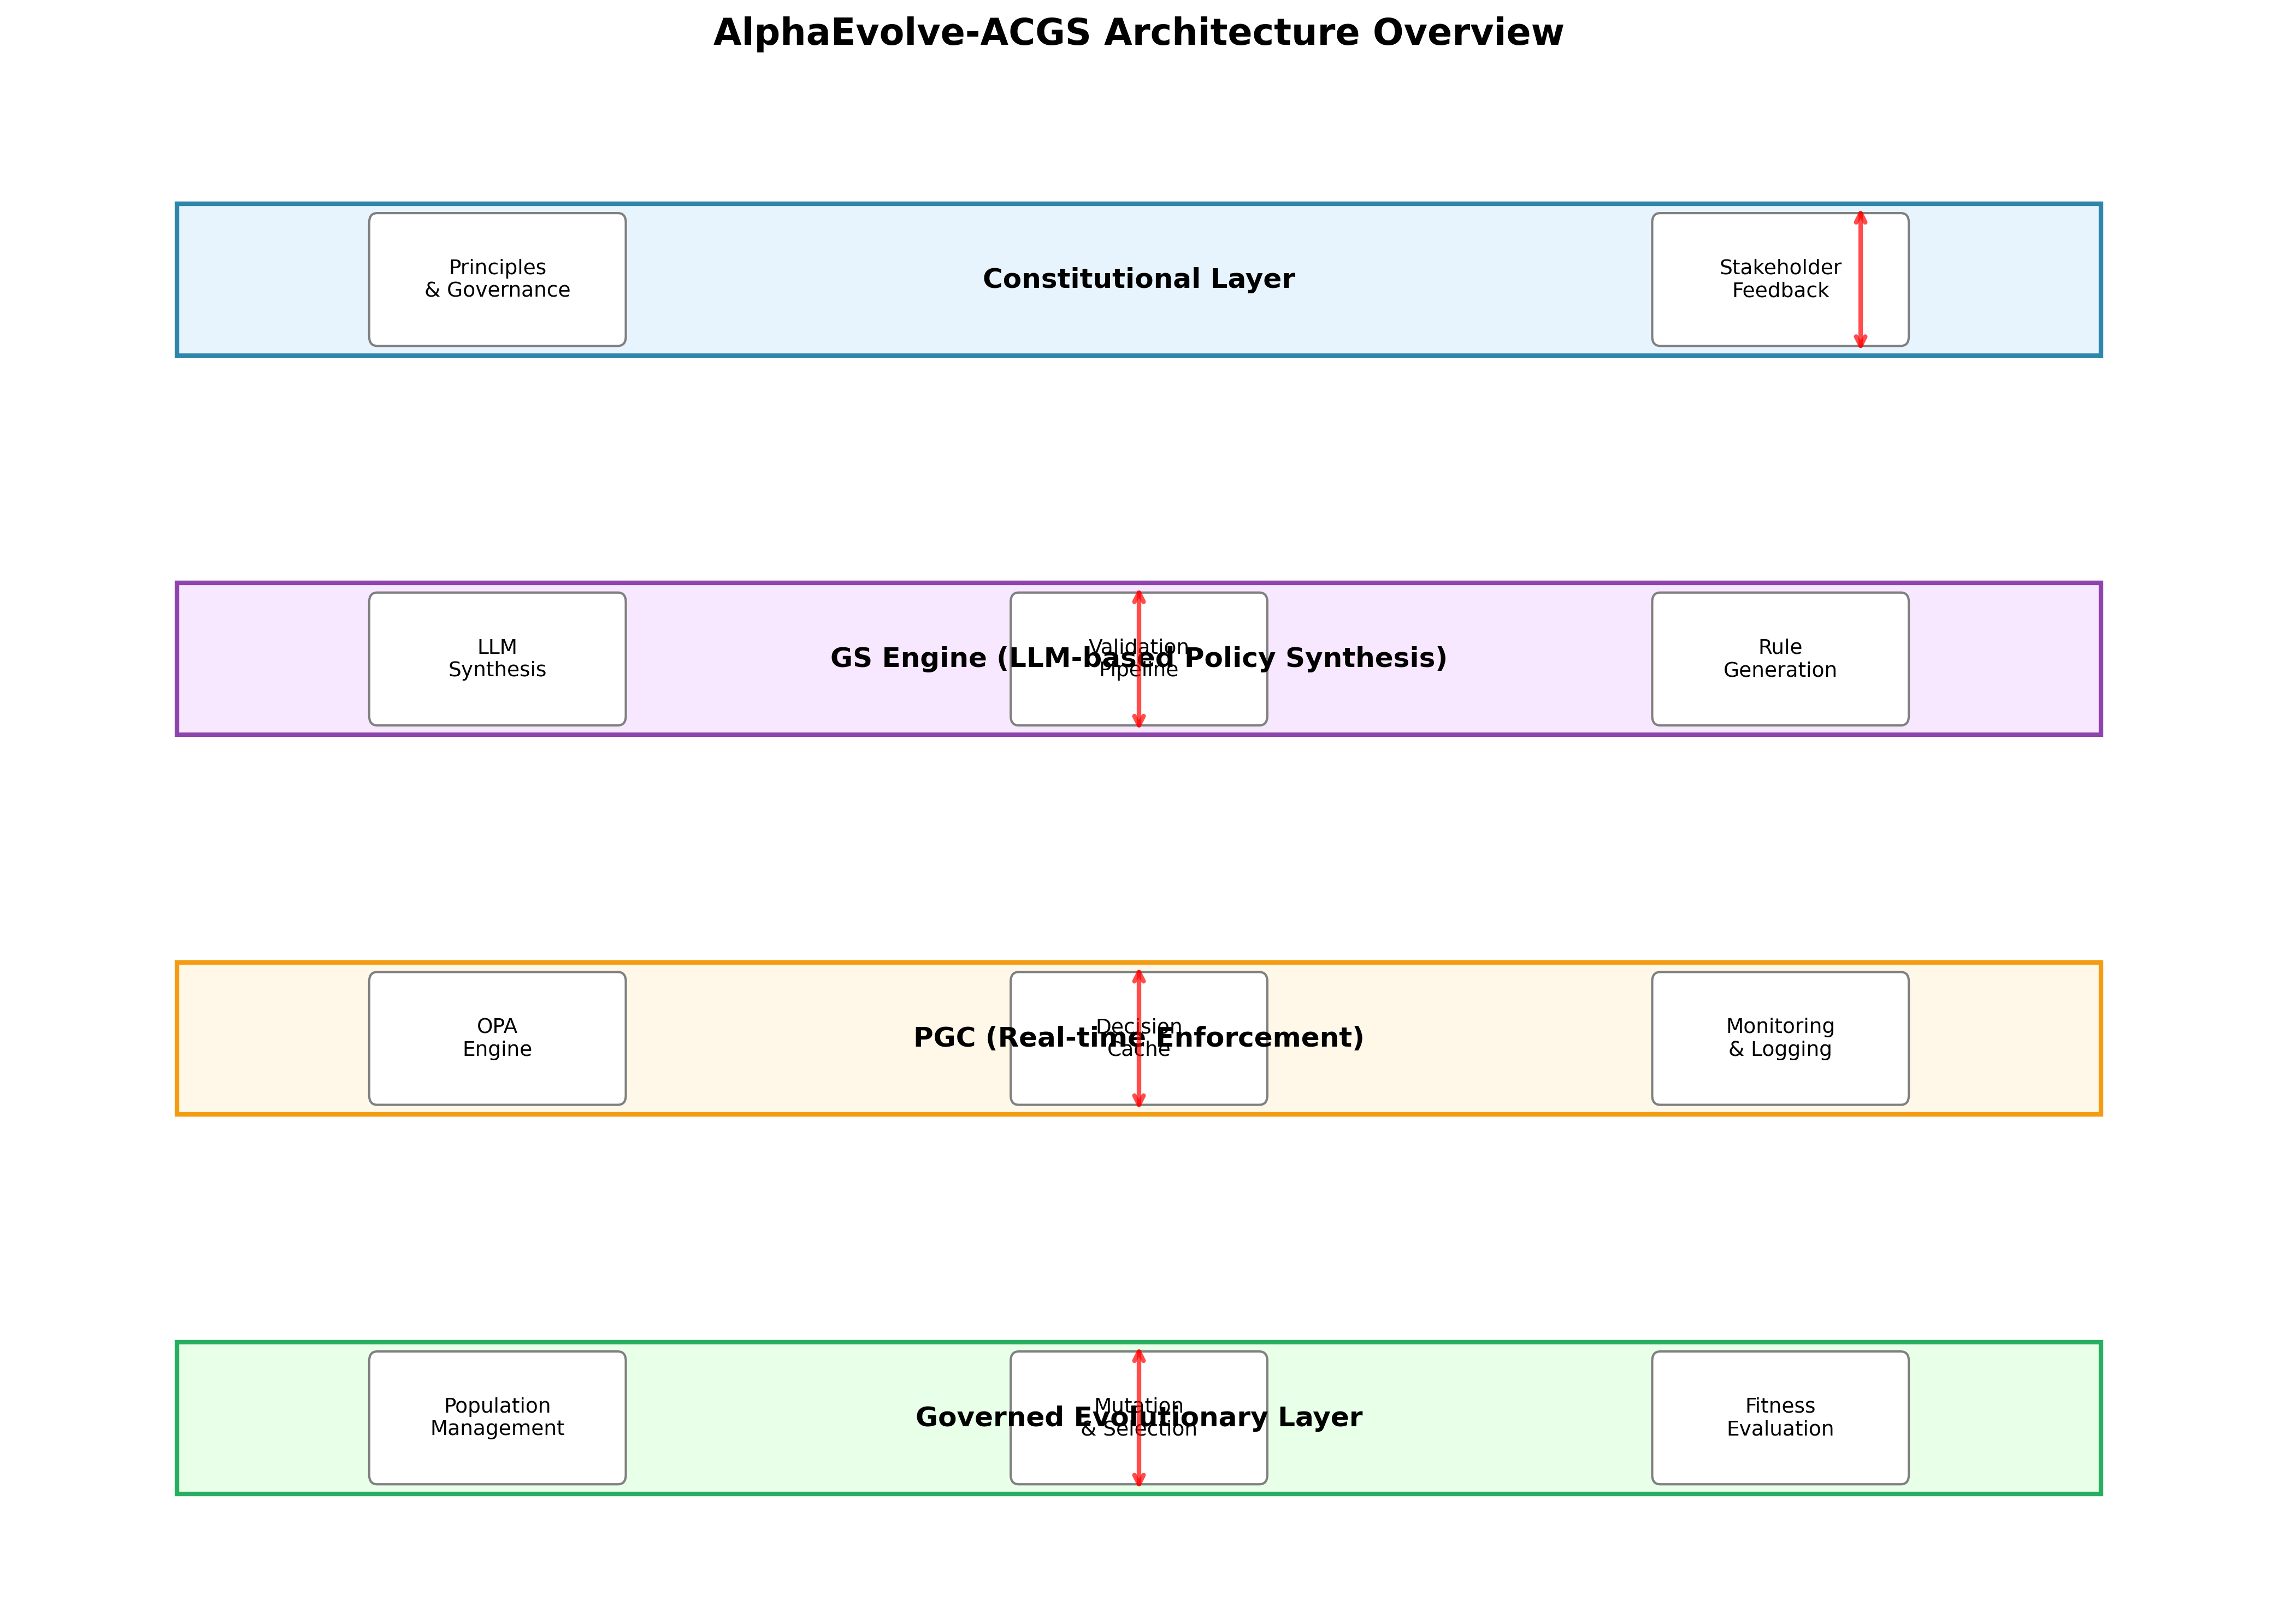
\includegraphics[width=\textwidth,height=0.35\textheight,keepaspectratio]{architecture_overview.png}
  \caption{Constitutional governance framework architecture showing four-layer integration: Constitutional Layer (principles and governance), GS Engine (LLM-based policy synthesis), PGC (real-time enforcement), and Governed Evolutionary Layer (constitutionally-aware EC). Feedback loops enable dynamic constitutional evolution.}
  \label{fig:teaser-architecture}
  % USER: Add \Description{} for accessibility if required by ACM.
  % \Description{Architectural diagram of the AlphaEvolve-ACGS framework, showing four interconnected layers: Constitutional, GS Engine, PGC, and Governed Evolutionary Layer, with feedback loops indicating co-evolution.}
\end{teaserfigure}

% --- Main Contributions ---
% Using the custom \contributionsbox command
\contributionsbox{%
\begin{enumerate}[itemsep=2pt,parsep=2pt,topsep=0pt,partopsep=0pt] % Adjusted list spacing
  \item[(1)] \textbf{Co-Evolutionary Governance Theory}: First formal framework where governance mechanisms evolve alongside AI systems, with mathematical foundations for constitutional adaptation and stability analysis (\Cref{sec:methods}).
  \item[(2)] \textbf{Real-Time Constitutional Enforcement}: Prompt Governance Compiler achieving \textbf{32.1ms} average latency with 99.7\% accuracy across three evaluation domains, enabling constitutional governance without performance degradation (\Cref{tab:pgc_comprehensive}).
  \item[(3)] \textbf{Automated Policy Synthesis Pipeline}: LLM-driven translation of natural language principles to executable policies with \textbf{68--93\%} success rates, including formal verification for safety-critical rules and multi-tier validation (\Cref{sec:synthesis_evaluation}).
  \item[(4)] \textbf{Scalable Democratic Governance}: Multi-stakeholder Constitutional Council with cryptographically-secured amendment protocols, formal appeal mechanisms, and demonstrated scalability to 50+ principles (\Cref{sec:governance_evaluation}).
  \item[(5)] \textbf{Comprehensive Empirical Validation}: Evaluation across arithmetic evolution, symbolic regression, and neural architecture search showing 94--97\% constitutional compliance with $<$5\% performance impact, plus head-to-head comparisons with baseline approaches (\Cref{sec:results}).
\end{enumerate}
}

% --- Terminology Glossary ---
% Using custom table commands
\begin{table}[h] % Consider [htbp] for more placement flexibility
  \centering
  \tablesize % Custom command for font size
  \caption{\textbf{Key Terminology and Acronyms}}
  \label{tab:glossary}
  \begin{tabularx}{\columnwidth}{@{}p{1.8cm}X@{}} % tabularx for fixed width with one expanding column
    \toprule
    \tableheader{Term} & \tableheader{Definition} \\ % Custom command for bold headers
    \midrule
    \tablenumfmt{ACGS} & AI Constitution Generation System (overall framework) \\ % Custom command for bold numbers/acronyms
    \tablenumfmt{AC Layer} & Artificial Constitution Layer (constitutional principles and governance) \\
    \tablenumfmt{CAI} & Constitutional AI \\
    \tablenumfmt{EC} & Evolutionary Computation \\
    \tablenumfmt{GS Engine} & Policy synthesis component within ACGS \\
    \tablenumfmt{HITL} & Human-in-the-Loop \\
    \tablenumfmt{LLM} & Large Language Model \\
    \tablenumfmt{OPA} & Open Policy Agent \\
    \tablenumfmt{PaC} & Policy-as-Code \\
    \tablenumfmt{PGC} & Prompt Governance Compiler \\
    \tablenumfmt{PoC} & Proof-of-Concept \\
    \tablenumfmt{RAG} & Retrieval-Augmented Generation \\
    \bottomrule
  \end{tabularx}
\end{table}

% --- Main Content Sections ---
\section{Introduction}
\label{sec:introduction}
Evolutionary computation (EC) systems represent a critical frontier in AI safety research, where traditional governance approaches fundamentally break down.
Unlike deterministic AI systems, EC generates emergent behaviors through population dynamics, mutation, and selection processes that cannot be predicted or controlled by static rule sets [Nordin2024LLMGP].
This creates what is termed the \textit{evolutionary governance gap}: the inability of existing AI governance frameworks to manage systems that continuously evolve their own behavior.
The comprehensive evaluation presented herein demonstrates the framework's effectiveness across multiple dimensions: LLM-driven policy synthesis achieves \textbf{68--93\%} success rates across complexity levels, scalability analysis with up to 50 constitutional principles shows sub-linear latency growth, and synthesis success rates maintain 89\% even at scale.
These results, combined with formal verification capabilities and democratic governance mechanisms, establish a robust foundation for constitutional AI governance.
Current approaches—from regulatory frameworks like the EU AI Act to technical solutions like Constitutional AI (CAI)—assume static or slowly-changing AI systems, rendering them inadequate for governing the dynamic, emergent nature inherent in evolutionary processes.
This paper presents a constitutional governance framework that embeds adaptive principles directly into evolutionary computation systems.
The proposed approach integrates two core components: an evolutionary computation engine and an AI Constitution Generation System (ACGS).
The ACGS utilizes Large Language Models (LLMs) to dynamically synthesize and adapt a \textit{living constitution}, which is encoded as executable policies and enforced in real-time by a Prompt Governance Compiler (PGC).
This architecture facilitates a co-evolutionary system where governance mechanisms and the AI system adapt in tandem, enabling what can be termed "constitutionally bounded innovation."
The framework addresses the verification gap often observed between natural language principles and their formal code implementations through multi-stage validation processes and iterative refinement loops.
While LLM-based policy generation inherently presents challenges regarding reliability, the proposed approach incorporates mechanisms designed to ensure semantic faithfulness and maintain constitutional integrity.
This work introduces five key contributions to the fields of AI governance and evolutionary computation:
\begin{itemize}[nosep,leftmargin=*] % nosep reduces space between items
    \item[\textbf{1.}] \textbf{Co-Evolutionary Governance Paradigm:} Introduction of the first governance framework designed to evolve concurrently with the AI system it governs. This addresses the fundamental mismatch between static governance models and dynamic AI behavior through a four-layer architecture that integrates constitutional principles, LLM-driven policy synthesis, real-time enforcement, and evolutionary computation.
    \item[\textbf{2.}] \textbf{LLM-to-Policy Translation Pipeline:} Development of a novel mechanism for the automated translation of natural language constitutional principles into executable Rego policies. This pipeline achieves \textbf{68-93\%} synthesis success rates across various levels of principle complexity and incorporates multi-tier validation, including formal verification for safety-critical rules.
    \item[\textbf{3.}] \textbf{Real-Time Constitutional Enforcement:} Demonstration of policy enforcement latencies below 50ms (32.1ms average), suitable for integration into evolutionary loops. This capability enables constitutional governance without compromising system performance, achieved through optimized Open Policy Agent (OPA)-based enforcement and intelligent caching strategies.
    \item[\textbf{4.}] \textbf{Democratic AI Governance Mechanisms:} Establishment of formal protocols for multi-stakeholder constitutional management. This includes a Constitutional Council structure, defined amendment procedures, appeal workflows, and cryptographic integrity guarantees, all designed to ensure democratic oversight of AI system governance.
    \item[\textbf{5.}] \textbf{Empirical Validation and Open Science:} Provision of comprehensive evaluation results demonstrating constitutional compliance improvements from approximately 30\% to over 95\% in evolutionary systems. The work is